\documentclass[11pt]{article}
\usepackage{macros}

\parindent0in
\pagestyle{plain}
\thispagestyle{plain}

\scribedby{Scribed By: Tao Huang}
\assignment{ShanghaiTech University, China}
\lecturedate{January 10, 2021}

\begin{document}
\maketitle

\outline{This note dedicates to conclude some important contents of Statistical Learning by Hang Li, augmented by some insights and self-understanding to them. The organization follows directly from Li, and I wish it can help you dive deeper in this interesting area. Let's start now!}\par

%%% Start writing and defining sections and subsections here
\tableofcontents
\clearpage
\section{Introduction to Statistical Learning}
\section{Perceptron}
\section{EM Algorithm}
\section{Hidden Markov Model}

% \begin{figure}[h]
%    \centering
%    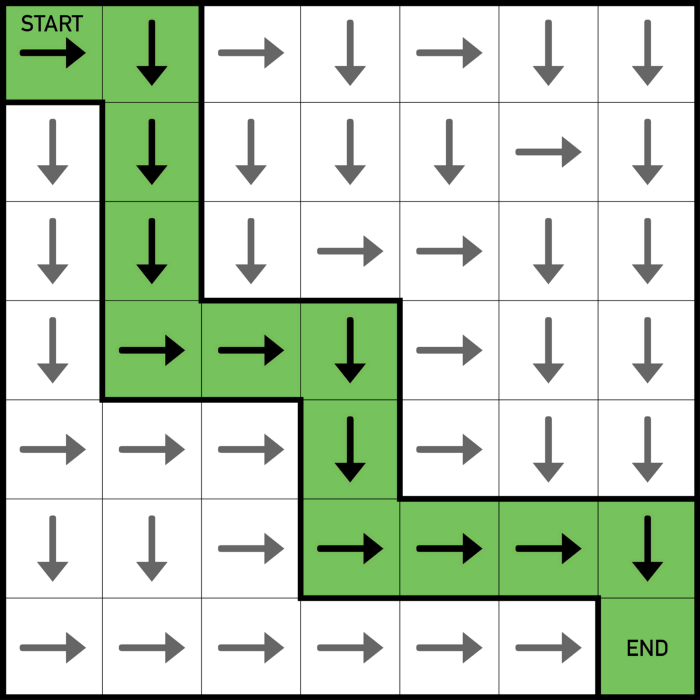
\includegraphics[width=0.5\linewidth]{assets/gridworld.png}
%    \caption{A sample figure depicting a gridworld}
%    \label{figure:gridworld}
% \end{figure}


%Keep figures (\texttt{.eps},\texttt{.jpg/png/etc},\texttt{.pdf}) and source codes inside the \texttt{assets/} folder. Please look at tthe source of Figure \ref{figure:gridworld} for reference.


\bibliographystyle{unsrt}
\bibliography{main}

\end{document}  